\chapter{Optomechanical topology optimization problems}
%\section{Opto-mechanical systems~\cite{ownpub1,ownpub2,ownpub3}}\label{sec:optomechanics}
Optomechanics, the study of the interaction between light and mechanical motion, is at the heart of state-of-the-art technologies, such as 
optical trapping~\cite{ashkin_acceleration_1970, moffitt_recent_2008} and cooling~\cite{cooling}, quantum information processing~\cite{Andrews_2014, Xi_2025}
, light sails~\cite{lightsail, lightsail1}, and high-precision metrology and sensing~\cite{sensing, weakforce, Li:18, Mason_2019}.

The most basic description of this interaction is given by the Lorentz force, which governs how moving charges respond to electric and magnetic fields:
\begin{equation}\label{eq:lorentz_f}
    \mathbf{\bm{\mathcal{F}}}(\mathbf{r},t) = q \left[ \bm{\mathcal{E}}(\mathbf{r},t) + \mathbf{v}(t) \times \bm{\mathcal{B}}(\mathbf{r},t) \right]\,,
\end{equation}
where $q$ is the charge and $\mathbf{v}$ is the velocity of the particle. This force can be generalized to describe more complex systems,
such as the the force between two current-carrying 
wires (Ampere's force law), and the electromotive force, which is at the core of many techologies, such as induction motors or generators.
In optomechanical systems, shaping the distribution and magnitude of these forces at the micro- and nanoscale is crucial for controlling mechanical motion with light. 
However, designing structures that can efficiently harness and manipulate these interactions often requires navigating highly complex
 parameter spaces and trade-offs between optical, mechanical, and material constraints.

To achieve such precise control, topology optimization has emerged as a a useful design technique enhance or tailor optomechanical interactions.
Recent advances include the design of coupling between optical and elastic
 waves~\cite{photo_topopt}, optical systems with nonlinear deformations~\cite{def_wg}, high-$Q$ optomechanical membranes~\cite{highQ1, fengwen, aragon1},
light sail structures~\cite{lightsail_topopt, lightsail_topopt1},
on-chip optical trapping devices~\cite{ownpub1}, particle design and manipulation~\cite{ownpub2, particle_opt},
and structural integrity constraint formulations~\cite{structural_integrity}
 among others.

 In the following subsections, we highlight our contributions to the field and review how to model optomechanical interactions in three distinct regimes: a general treatment based on the Maxwell stress tensor~\cite{ownpub2}; 
 the dipole approximation for small particles~\cite{ownpub1, ownpub3}; and strongly coupled systems where optical forces can induce significant mechanical deformations.
\section{The Maxwell Stress Tensor formalism~\cite{ownpub3}}

In the most-general case, the optical force can be calculated using the Maxwell stress tensor (MST) formalism, which can be derived from the generalization of the Lorentz force (\eqref{eq:lorentz_f}) in continuous media~\cite{novotny}.
The basic idea is sketched in \figref{fig:eng_res}, where
a particle scatters an incident electromagnetic field $\mathbf{E}_\text{inc}$ creating the scattered field $\mathbf{E}_\text{scat}$ and the net force $\mathbf{F}$ that acts
on the particle. The time-averaged net force is given by
\begin{equation}\label{eq:f_MST}
    \langle\bm{\mathcal{F}}\rangle=\int_{\partial V}\langle\stackrel{\leftrightarrow}{\bm{\mathcal{T}}}(\mathbf{r}, t)\rangle \cdot \mathbf{n}_{\partial V}(\mathbf{r}) \d \mathbf{r}\,,
\end{equation}
where $\partial V$ denotes any boundary enclosing the particle, $n_{\partial V}$ denotes the unitary vector normal to that boundary, and
the stress tensor is given by:
\begin{equation}
    \begin{aligned}
        \stackrel{\leftrightarrow}{\bm{\mathcal{T}}}(\mathbf{r}, t)= & {\left[\varepsilon_0 \varepsilon_r \mathcal{E}(\mathbf{r}, t) \otimes \mathcal{E}(\mathbf{r}, t)+\mu_0 \mu_r \mathcal{H}(\mathbf{r}, t) \otimes \mathcal{H}(\mathbf{r}, t)\right.} \\
    & \left.-\frac{1}{2}\left(\varepsilon_0 \varepsilon_r \mathcal{E}^2(\mathbf{r}, t)+\mu_0 \mu_r \mathcal{H}^2(\mathbf{r}, t)\right) \stackrel{\leftrightarrow}{\mathbf{I}}\right],
    \end{aligned}
\end{equation}
where $\otimes$ denotes the outer product. Note that the permittivity and permeability correspond to those of the medium surrounding the particle.

\begin{figure}[tb]
    \centering
    \makebox[\textwidth][c]{\includegraphics{figures/eng_results.png}}%%
    \caption{Topology optimization in optical force applications. (a) A scattering particle 
    enclosed by a boundary $\partial V$ scatters a field $\mathbf{E}_\text{scat}$, when excited by an incident field $\mathbf{E}_\text{inc}$, 
    generating a net optical force $\mathbf{F}$. (b) Electric-field intensity distribution for a particle design optimized to maximize the vertical ($y$)
    component of the optical force. Adapted with permission from~\cite{ownpub2} \copyright Optical Society of America.}
    \label{fig:eng_res}
\end{figure}

\subsection*{Engineering optical forces via topology optimization}

In~\cite{ownpub3} we use this formalism to optimize the geometry of particle-metalens pairs for difference applications, such as attracting, repelling, 
oscillating and trapping particles. In \figref{fig:eng_res} we depict an example optimization result from our work, where 
we optimize the geometry of a particle to maximize the vertical component of the optical force by maximizing $\text{FOM} = \langle\bm{\mathcal{F}}\rangle \cdot \mathbf{n}_y$, where
in our two-dimensional example $\mathbf{n}_y = (0, 1)$ is the unitary vector in the vertical direction.  Our results show that the optimized particle geometry is a Bragg-mirror-like
structure, which is able to efficiently reflecting the incoming plane-wave, resulting in a efficient exchange of force and momentum. In the remainder of~\cite{ownpub3} we extend this example by also designign a metalens to focus the incoming plane-wave onto the particle,
we design attractive particle geometries, and optical-tweezer like setups to trap the particle in space. All the code developed in this work is available on GitHub~\cite{github_MST} with examples on force calculation and topology optimization. 

One interesting aspect of the topology optimization of particles in the MST formalism is that with our current framework the particle cannot feature disconnected members; otherwise
one would need to integrate around the individual components to calculate the total force for each one. It is possible to get around this by enforcing 
a connectivity constraint via the VTM~\cite{li_structural_2016}(see \secref{sec:thermo_optical}). In our examples
we enforce particle connectivity to the center of the design domain, and also of the metalens structure to the bottom, as to ensure Structural
integrity of the structure.

\subsection*{Outlook and future work}

This optimization work is the first, to our knowledge, to 
consider the MST formalism, paving the way for future work in three-dimensional systems and more complex optimization problems, such as optically-driven particle
trajectory control~\cite{zemanek_perspective_2019, macdonald_microfluidic_2003, shilkin_directional_2017}, many-body particle systems~\cite{bechinger_active_2016, chang_colloquium_2018} or optically actuated devices~\cite{ivanyi_optically_2024}, among others.
Finally, it is worth noting that a particularly interesting and straightforward extension would be to use the MST formalism to calculate the time-averaged torque acting on a particle, defined as~\cite{novotny}
\begin{equation}
    \langle \bm{\tau} \rangle = \langle \mathbf{r} \times \bm{\mathcal{F}} \rangle = \int_{\partial V} \langle \mathbf{r}
     \times \stackrel{\leftrightarrow}{\bm{\mathcal{T}}} \rangle \cdot \mathbf{n}_{\partial V} \d\mathbf{r} 
\end{equation}
where $\mathbf{r}$ is the vector defimed between the rotation axis and force application point. This definition of torque accounts
for two kinds of rotational motion; \textit{spinning} ($\langle \bm{\tau}_S \rangle$), where the particle rotates around its center of mass,
and \textit{orbiting} ($\langle \bm{\tau}_O \rangle$), where the particle rotates around an external axis, so that the total torque is the sum
of both the spin and orbital torque $\langle \bm{\tau} \rangle = \langle \bm{\tau}_S \rangle + \langle \bm{\tau}_O \rangle$~\cite{torque}.  Defining
and optical torque-based FOM could open the door for the design of efficient optical and biological micro- and nanomachines~\cite{rotating}.

\section{The dipole approximation~\cite{ownpub1, ownpub3}}

When particles are much smaller than the wavelength of the electromagnetic field ($s\ll \lambda$), it is possible to model the optical force via the dipole approximation in the
quasistatic limit. In this approximation, the particle is treated as a point dipole with a polarizability $\alpha$, which describes how the particle responds to the local electric field frequency-domain $\mathbf{E}$.
In the dipole approximation the optical force on the particle can be expressed as~\cite{novotny}:
\begin{equation}
    \langle\mathbf{F}\rangle=\overbrace{\frac{\alpha^{\prime}}{4} \nabla\left\{\mathbf{E}^* \cdot \mathbf{E}\right\}}^{(1)}
    +\frac{\alpha^{\prime \prime}}{k \varepsilon_0} \Big[\overbrace{\frac{1}{c}\langle \mathbf{S} \rangle}^{(2)} + \overbrace{c \left( \nabla \times \langle \mathbf{L} \rangle \right)}^{(3)}\Big]\,,
\end{equation}
where the polarizability can be split up into the real and imaginary parts 
$\alpha=\alpha^\prime + i \alpha^{\prime \prime}$, the Poynting vector is given by $\mathbf{S} = \mathbf{E} \times \mathbf{H}$, and the time-averaged angular momentum is 
$\langle \mathbf{L} \rangle = [\varepsilon_0/(4 i \omega)](\mathbf{E} \times \mathbf{E}^*)$. 
The term associated with the Poynting vector is the radiation pressure ($2$), while the term associated 
with the angular momentum ($3$) is the spin-curl force.

In the abscence of absorption effects ($\alpha^{\prime \prime}=0$), the force is totally described 
by the gradient force ($1$), which is a conservative force that can be described as the gradient 
of a trapping potential:
\begin{equation*}
    U (\mathbf{r}) = -\frac{\alpha^{\prime}}{4} \left|\mathbf{E}(\mathbf{r})\right|^2\,.
\end{equation*}
where the force can be calculated as $\mathbf{F} = -\nabla U(\mathbf{r})$. 
For non-resonant and non-absorbing isotropic particles the polarizability is 
described through the relation~\cite{BornWolf:1999:Book}
\begin{equation}
    \alpha^{\prime}= 3 \varepsilon_0 $V$ \frac{\varepsilon_p-\varepsilon_m}{\varepsilon_p+2 \varepsilon_m}\,,
\end{equation}
where $V$ is the volume of the particle, $\varepsilon_p$ and $\varepsilon_m$ are the
dielectric constants of the particle and the medium, respectively. Note that in the dipole approximation do not consider the particle modifying
the optical field, which works well for point-like particles in free-space but not necessarily 
for either large particles, particles with high refractive contrast, or particles close to material
boundaries (e.g., optical cavities). This interaction can be accounted for in the dipole
approximation by considering the self-induced back-action (SIBA) effect, which assumes a weak
perturbation of the field due to the particle and expands the field in terms of 
the scattering Green function of the particle, which leads to a self-consistent
equation for the total electric field which can be used to calculate the force~\cite{novotny, SIBA, benjamin}. If the series converges this leads 
to same result as the MST calculation (\eqref{eq:f_MST}), which is often used to validate the dipole approximation (e.g., \cite{ownpub1,ownpub3}). 

\subsection*{On-chip omnidirectional optical trapping via topology optimization~\cite{ownpub1}}

Using the dipole approximation formalism in~\cite{ownpub1} we use topology optimization to design an integrated omnidirectional optical trapping chip, which is able to trap particles in three dimensions,
which was previously only possible with the use of free-space optical tweezers~\cite{ashkin_acceleration_1970}, or bulky photonic devices~\cite{manka_simulation_2024}. This is done by minimizing 
the difference of the electric-field norm with respect to a reference field $\mathbf{E}_\text{ref}$:
\begin{equation}
    \text{FOM} \equiv \Phi=\sqrt{\int_{\Omega}\left[\Theta\left(\frac{|\mathbf{E}(\mathbf{r})|}{\left|\mathbf{E}\left(\mathbf{r}_0\right)\right|}-\frac{\left|\mathbf{E}_{\text{ref}}(\mathbf{r})\right|}{\left|\mathbf{E}_{\text{ref}}\left(\mathbf{r}_0\right)\right|}\right)\right]^2} \text{~d} \Omega
    \end{equation}
where the fields are normalized with respect to the value at the center of the design domain $\mathbf{r}_0$, and $\Theta$ is the smoothed Heaviside threshold, which ensures
potentials as steep or steeper than the reference. The reference is chosen as a Gaussian trapping potential, but can be any other potential, such as a harmonic potential ($U\propto\mathbf{r}^2$).

By applying this optimization framework we obtain the topology-optimized cavity design in \figref{fig:MST_dipole}, which is able to trap particles at the center of an optical
cavity in three dimensions and has an associated Gaussian-like trapping potential, with a depth  $U<-10\, k_B T$ at room temperature ($T=300$ K) conventionally needed to overcome Brownian fluctuations~\cite{novotny}.
As long as the dipole approximation is valid one can tune the input power to trap paricles of arbitrarily small sizes.

\begin{figure}[tb]
    \centering
    \makebox[\textwidth][c]{\includegraphics{figures/MST_dipole.png}}%%
    \caption{Optical response and trappig potential for the topology-optimized particle trap. (a) Lower half ($z<0$) of the optimized cavity, with the electric-field intensity
    distribution when excited with the fundamental waveguide mode at $\lambda=1.55$ \textmu m. (b) Trapping potential for a $R=15$ nm and $n=2$ particle in the cavity region for the different axial line- and plane-cuts as a function
    of the distance from the center ($d$), with the stable trapping regime ($U<-10 k_B\, T$) highlighted in gray. Adapted with permission from~\cite{ownpub1}.}
    \label{fig:MST_dipole}
\end{figure}

From the dipole approximation trapping potential we calculate the the force-displacements curves and we determine trapping stiffnesses
of $\kappa \approx 0.5$ fN/nm, an order of magnitude larger that diffraction-limited free-space optical tweezers~\cite{ownpub1}. To validate this findings
we employ the MST formalism to calculating the force on spherical particles as they are displaced from the cavity center in the axial directions, and find excellent
agreement with the dipole approximation. As shown in \figref{fig:SPIE}, to further verify the the dipole approximation assumption in ~\cite{ownpub3} we compare the results of the dipole approximation with the MST
for varying particle sizes and refractive indices, showing that the dipole approximation is a good approximation
even for large values of the refractive index (e.g., $n=3$) and particle sizes up to $s\approx 0.05 \lambda$. As we can see for larger sizes and refractive indices 
the results start to deviate, and the dipole approximation should break down for even larger values.

\begin{figure}[tb]
    \centering
    \makebox[\textwidth][c]{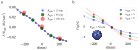
\includegraphics{figures/SPIE_results.png}}%%
    \caption{Validating the dipole approximation force (dashed line) against the MST force (data points), for the force as a function of displacement ($d$) from the cavity center.
    (a) Volume-normalized force ($F/R^2_\text{sph}$) for different particle sizes with refractive index $n_\text{sph}=2$. (b) Force for different refractive indices of the particle for a particle radius $R_\text{sph}=50$ nm. Adapted from~\cite{ownpub3}.}
    \label{fig:SPIE}
\end{figure}

\subsection*{Benchmarking trapping performance~\cite{ownpub1}}

When designing optical trapping platforms it is important to be able to compare performance across platforms. To this end, in~\cite{ownpub3} we introduce a normalized
trapping stiffness metric, which normalizes trapping stiffness to particle  polarizability and input power ($P_\text{in}$)
\begin{equation}
    \eta_i=\frac{\kappa_i \varepsilon_0}{\alpha^\prime P_{\text{in}}}
\end{equation}
enabling one-to-one comparison across trapping devices\footnote{As noted in~\cite{ownpub3} this metrics breaks down for lightless platforms (e.g., Casimir force-based traps), and the metric could be redefined
without including the input power.}. The normalized trapping stiffness allows us to show that (Tab. 1 in~\cite{ownpub3}), although plasmonic devices can reach higher normalized 
stiffnesses, they suffer from optical losses to heating and lack omnidirectional stability. In contrast, our inverse-designed dielectric platform
 achieves comparable normalized stiffnesses to other dielectric traps while uniquely offering fully stable, omnidirectional trapping
  without relying on SIBA effects. Notably, SIBA-based devices are particle-specific and their performance can break down
   for different particle geometries or materials. Compared to conventional optical tweezers, our device maintains similar trapping
    strength at lower input power due to its integrated, waveguide-coupled design, highlighting the benefits of miniaturized,
     near-field-based optical trapping.

\subsection*{Outlook and future work}

Lastly, in~\cite{ownpub2} we also discuss the effects of Casimir Polder effects on particle loading into the trap, and
also discuss possible applications of our proposed devices in particle optomechanics and
biophotonics, where the ability to control a trapped particle omnidirectionally in a compact integrated device
couled lead to novel technological applications. ADD SOME CONCLUSION, APPLICATIONS.

\section{Strongly coupled optomechanical systems}\label{sec:mech_strongly_coupled}

Mechanical steady-state force balance
\begin{equation}
    \nabla \cdot \overleftrightarrow{\boldsymbol{\sigma}} + \mathbf{f} = 0\,,
\end{equation}
Stress tensor:
\begin{equation}
    \nabla \cdot \overleftrightarrow{\boldsymbol{\sigma}} + \nabla \cdot \overleftrightarrow{\mathbf{T}} = 0\,,
\end{equation}

In strongly coupled optomechanical systems, the optical field can significantly modify the mechanical properties of the system, leading to a significant deformation
of the device, which in turn modifies the optical response. 

We have studied these systems in terms of topology optimization, as part of some unpublished work. In this work we consider 
the mechanical deformation of a membrane-like system, which is optically excited by a plane-wave. The optical field is calculated using the MST,
and the mechanical deformation is calculated using the linear elasticity theory. The mechanical deformation is then used to modify the optical field, 
leading to a self-consistent problem that can be solved iteratively, similar to other work.

ADD SOME OF THE WORK WITH THE MEMBRANE-LIKE SYSTEM HERE. TO BE FINISHED!
